\documentclass[12pt]{article}
\usepackage{latexsym}
\usepackage{epsfig}
\usepackage{amsmath}
\usepackage{amssymb}


\setlength{\topmargin}{0in}
\setlength{\leftmargin}{0in}
\setlength{\textwidth}{6in}
\setlength{\textheight}{9.5in}
\setlength{\parindent}{0.2in}
\setlength{\parskip}{.08in}
\voffset = -.45in
\hoffset = -.5in
\newcommand{\lsp}[1]{\large\renewcommand{\baselinestretch}{#1}\normalsize}

\begin{document}

\lsp{1}
\pagestyle{plain}
\begin{center}
{\bf
Graph Representation Worksheet
}
\end{center}

\begin{figure}[h]
\center
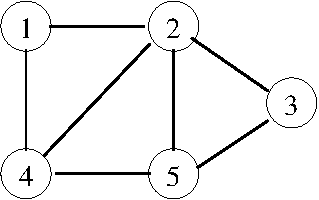
\includegraphics[width = 2in]{adjacency.pdf}
\end{figure}

\begin{enumerate}
\item What are the storage requirements assuming an adjacency matrix
is used. Assume each element of the adjacency matrix requires four 
bytes.

\vspace*{1in}

\item Repeat for an adjacency list representation. Assume that an 
{\bf int} requires 4 bytes and that a pointer also requires 4 bytes.

\vspace*{1in}

\item Now, consider an undirected graph with 100 vertices and 1000 edges. 
What are the storage requirements for the adjacent matrix and adjacency
list data structures?
 
\end{enumerate}
 

\end{document}
